
% Template file for ACCV 2009
%\documentclass[runningheads]{llncs}
%In order to omit page numbers and running heads
%please use the following line instead of the first command line:
\documentclass{llncs}
%Furthermore change the line \pagestyle{headings} to
%\pagestyle{empty}
\usepackage{graphicx}
\usepackage{subfig}
\usepackage{amsmath}

\begin{document}

%\pagestyle{headings}
%In order to omit page numbers and running heads
%please change this line to
\pagestyle{empty}
%and change the first command line too, see above.

\mainmatter

\title{Lightweight 3D Reconstruction of Urban Buildings From Range Data}

\titlerunning{Lecture Notes in Computer Science}

%\author{Alfred Hofmann\inst{1}
%\and Ingrid Beyer\inst{1} \and
%Anna Kramer\inst{1} \and Erika Siebert-Cole\inst{1} \and\\
%Angelika Bernauer-Budiman\inst{2} \and
%Martina Wiese\inst{2} \and Anita B\"urk\inst{3}}
%
%\authorrunning{Alfred Hofmann et al.}

\author{}



%\institute{Springer-Verlag, Computer Science Editorial III,
%Postfach 10 52 80,\\
%69042 Heidelberg, Germany\\
%\email{\{Hofmann, Beyer, Kramer, Erika.Siebert-Cole, LNCS\}@Springer.de}\\
%\texttt{http://www.springer.de/comp/lncs/index.html}
%\and
%Springer-Verlag, Computer Science Production, Postfach 10 52 80,\\
%69042 Heidelberg, Germany\\
%\email{\{Bernauer, Wiese\}@Springer.de}
%\and
%Springer-Verlag, Marketing Management, Postfach 10 52 80,\\
%69042 Heidelberg, Germany\\
%\email{Buerk@Springer.de}}

\institute{Paper ID: 432}

\maketitle

\begin{abstract}
Laser range scanners are widely used to acquire accurate scene measurements.
The massive point clouds they generate, however, present challenges to
efficient modeling, visualization, and storage.
State-of-the-art techniques for generating 3D models from voluminous
range data is well-known to demand large computational and storage requirements.
In this paper, attention is directed to the modeling of urban buildings
directly from range data.
We present an efficient modeling algorithm that exploits \emph{a priori}
knowledge that buildings can be modeled using extrusion and taper operations
to cross-sectional contours.
Inspired by this simplicity, we identify key cross-sectional slices among
the point cloud that consist of salient features.
Standard image processing algorithms are used to remove noise, fill holes,
and vectorize the projected points into contours.
Applying extrusion and taper operations to these contours
permits us to achieve dramatic geometry compression, making the resulting
models suitable for web-based applications such as Google Earth
or Microsoft Virtual Earth.
This work has applications in architecture, urban design, virtual city
touring, and online gaming.
We present experimental results on the exterior and interior of urban building
datasets to validate the proposed algorithm.
\end{abstract}

\section{Introduction}
Automatic 3D modeling of urban buildings is an area of active research
with increasing attention drawn from the computer graphics and
computer vision communities.
Current state-of-the-art algorithms for 3D modeling of urban buildings are
computationally expensive and suffer under the weight of large-scale datasets.
Despite a recent thrust of activity in 3D modeling and visualization of
urban buildings for web-based applications such as Google Earth and Microsoft
Virtual Earth, much 3D modeling continues to be manually generated.
Applications such as Google SketchUp are popular tools for creating
3D models of urban buildings via an intuitive push-pull modeling interface.
This process, however, remains tedious, expensive, and generally produces
low-resolution results.
This paper seeks to introduce an automatic and efficient algorithm for
generating lightweight 3D models of urban buildings directly from point clouds.

The proposed algorithm can generate models across a wide spectrum of
resolutions.
A particularly useful feature of the algorithm is that even for a low
resolution model, the sharpness of the raw data is preserved, thereby
outperforming most of the existing approximation techniques.
The contribution of this work is that it combines the benefits of
\emph{a priori} knowledge of urban buildings and lightweight 2D image
processing techniques to perform 3D modeling of urban buildings directly
from point cloud data.
This offers the benefit of a cost-effective geometry compression
approach for voluminous range data.
It can be applied to boost web-based 3D applications, including
Google Earth, Microsoft Virtual Earth, virtual city touring and online gaming.

%\section{Previous Work}
In an attempt to steer clear of tedious and expensive hand-made models,
procedural modeling of buildings in \cite{PMB_MWH,PMB_WWS} has been proposed.
By using an effective description language, buildings and streets of a virtual
city can be generated automatically.
The strength of this approach is that the description language can generate
a huge number of buildings and streets quickly and beautifully.
This is particular useful for gaming or other computer graphics applications.
However, since the parameters used to generate the buildings are randomly
generated, the city generated with these buildings and streets is a virtual one.
This approach is not useful for attempting to model an {\it existing} building.
In order to do so, one has to manually specify the parameters of the building,
which is very cumbersome.
Our goal is to automatically infer the parameters of an existing building and
therefore reproduce it quickly using the procedural modeling language
described above.

There has been a lot of related work on 3D reconstruction in the research
community.
Essentially, this reconstruction process is the reverse engineering problem
of computer graphics \cite{RE_Fisher}.
Reverse engineering of range data has been applied in numerous research areas,
including computer-aided design (CAD), computer vision, architectural modeling,
and medical image processing.
In \cite{RE_TOGSH}, Thompson et al. made use of known manufacturing features
to infer the 3D structure of the mechanical parts.
Their method benefits from the domain knowledge that most of the mechanical
parts consist of predefined structures, such as holes, bosses, and grooves.
Our work is partially motivated by this idea since it also incorporates
{\it a priori} knowledge about the construction of urban buildings for further
inference.
However, their method is based on predefined simple geometry structures and
the assumption that the input 3D data has a high signal-to-noise (SNR) ratio.
This hinders their approach for those applications with low SNR and
incomplete data.

\begin{figure} [!btp]
  \subfloat[]{
    \label{fig_IR_2_DXF:a} %% label for first subfigure
    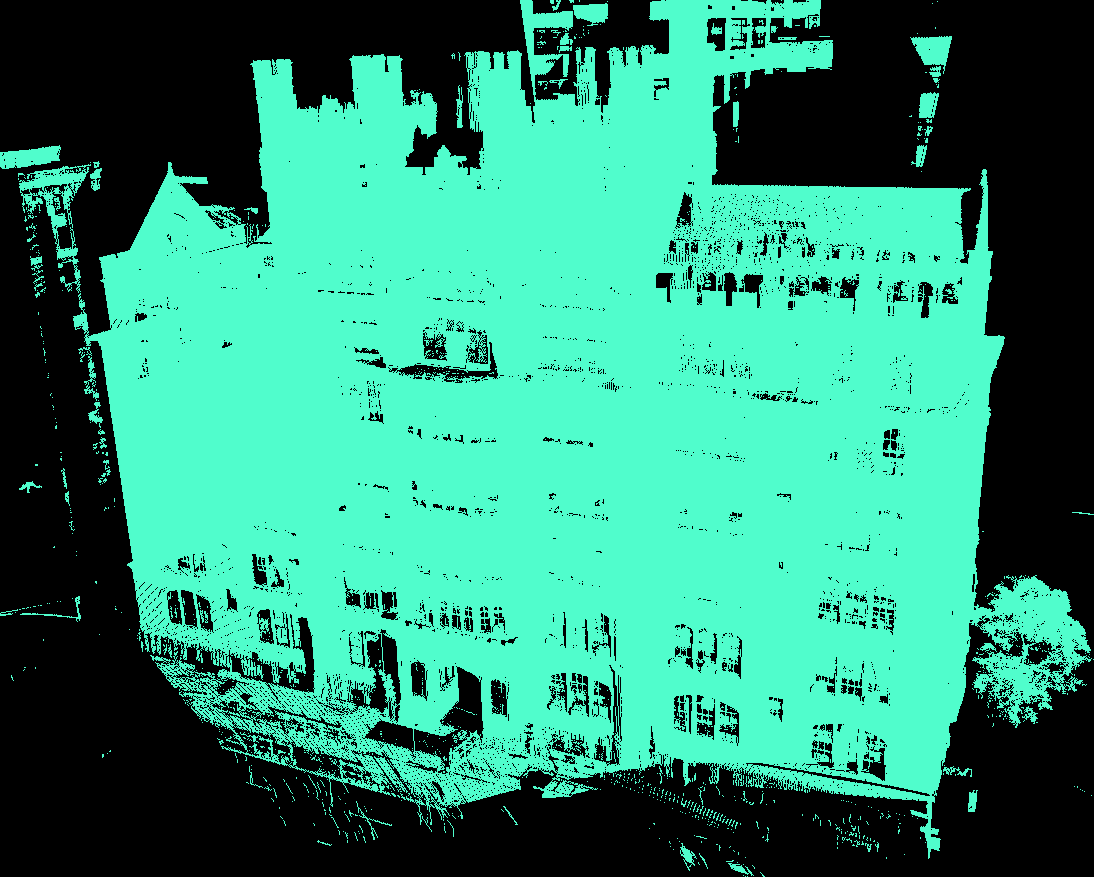
\includegraphics
        [width=1.5in]
	{figures/point_cloud.png}
  }
  \subfloat[]{
    \label{fig_IR_2_DXF:d} %% label for first subfigure
    \includegraphics
        [width=1.5in]
	%{figures/IR_skp_face_1000_4_1_paper.png}
	{figures/HunterShaded.jpg}
  }
  \subfloat[]{
    \label{fig_GE} %% label for first subfigure
    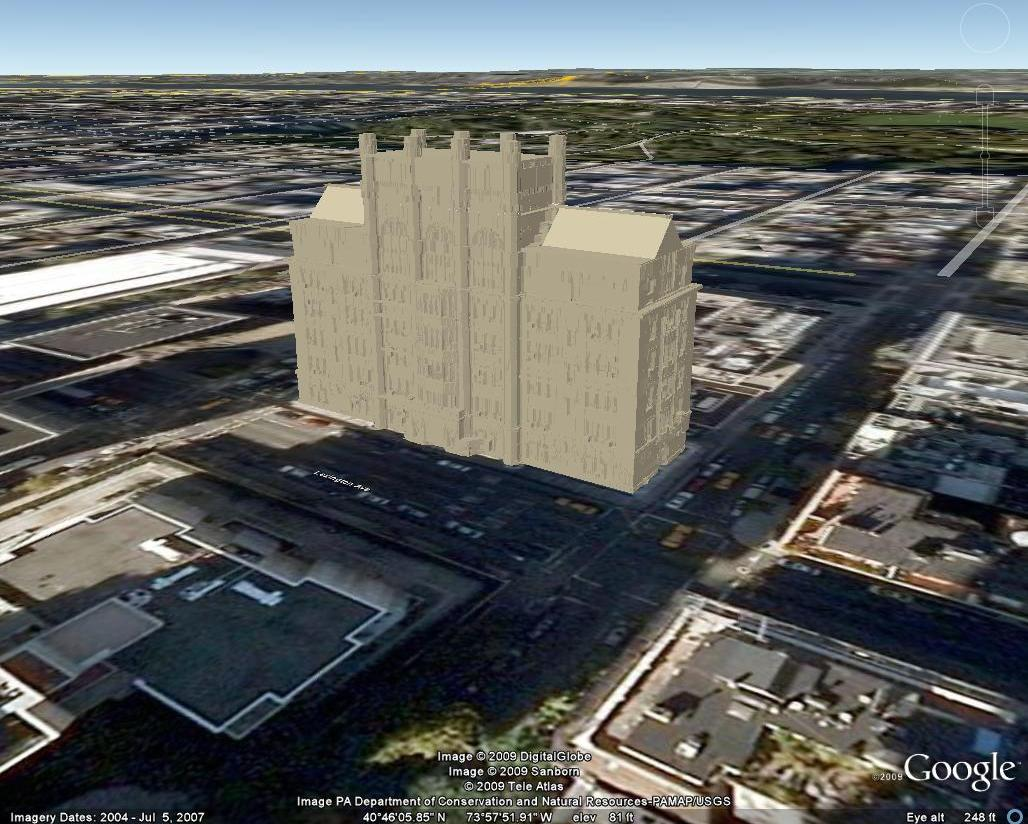
\includegraphics
        [width=1.5in]
	{figures/HunterGE.jpg}
  }
  \caption{
(a) A snapshot of the 3D point cloud assembled by registering multiple scans.
%(b) wire-frame model of the building.
%(c) colored layer model of the building.
%(d) white face model of the building.
(b) The lightweight 3D model of the point cloud data reconstructed by our proposed algorithm.
(c) The placement of the 3D model on Google Earth.
}
  \label{fig_IR_2_DXF}
\end{figure}
%%% End of Figure

Medical image processing techniques, on the other hand, usually deal with
low SNR data.
There has been a lot of work on medical 3D image reconstruction.
The basic idea behind the vast amount of work conducted in this area is 3D
reconstruction from sliced or histologic images using interpolation techniques.
Statistical inference is also extensively used to infer the low SNR images.
For example, in \cite{MIR_FJS}, Sigworth addressed the problem of low SNR
images using the maximum-likehood approach.
Most of these statistical processes are computationally intensive
in order to obtain accurate, high resolution models.

We propose an efficient way to reconstruct 3D models from range data by
partitioning the data into thin cross-sectional slabs of volume.
For each slab, all range data in that slab is projected onto a 2D
cross-sectional image slice.
Producing this array of slices permits us to avoid direct computation on
3D data, which is time-consuming and computationally complex.
A similarity measure \cite{IR_Brown} can be used to cluster the sliced images
together into {\it keyslices}.
This term is analogous to ''keyframes'' in computer animation, which denote
important moments in the animation sequence from which intermediate results
can be derived.
Each keyslice is a 2D image which contains the salient cross-sectional
structure of a building.
We leverage fast 2D image processing techniques on these keyslices
to produce lightweight 3D models, consisting of only a few hundred polygons.

%%%%%%%%%%%%%%%%%%%%%%%%%%%%%%%%
%%%%%%   PREPROCESSING  %%%%%%%%
%%%%%%%%%%%%%%%%%%%%%%%%%%%%%%%%
\section{Preprocessing the Range Data}
\label{sec_prep}
The input to our system is range data assembled as a 3D point cloud.
Our data is obtained from a Leica Cyrax 2500 laser range scanner \cite{RDP_LRS},
which works by sweeping an eye-safe laser beam across the scene to collect
up to one million 3D depth points per frame.
All scene points that lie within 100 meters can be acquired with an accuracy
of 5mm in depth.
The basic algorithm that we use for registering the voluminous 3D data
acquired from multiple scans of buildings has been introduced in
\cite{RDP_LS}.
Figure \ref{fig_IR_2_DXF}\subref{fig_IR_2_DXF:a} shows a snapshot of the
registered 3D point cloud, consisting of 14 scans totalling 14 million points.

Due to occlusions and limited vantage points, the point cloud collected by the
laser scanner \cite{RDP_LRS} contains noise and missing data.
In addition, computing directly on 3D data is time-consuming and
computationally complex.
To tackle these issues, we define inner and outer bounding boxes for the
building to clip away unrelated scene objects.
Then, we convert the 3D modeling problem into a set of 2D problems by
projecting the 3D data into a series of 2D cross-sectional images.
Noise removal, hole filling, and vectorization are all done in this
2D space.

\subsection{Extraction of 2D Slices}
\label{sec_image_slicing}
We consider the point cloud data as a large array of 3D points that can be
sliced into horizontal slabs of volume.
All 3D points within each slab will be projected onto a horizontal cutting
plane, or slice, at the base of the slab.
The height of each slab is $\boldsymbol{\delta}$.
If that value is held constant, each slice is generated from equal-sized
slab intervals.
If $\boldsymbol{\delta}$ is allowed to be a dynamic value, then we may
choose to allow for large values in parts of the structure that are similar,
and low values in regions that contain finer detail.
To avoid working on 3D data directly, a relatively small constant value
for $\boldsymbol{\delta}$ is chosen to generate 2D cross-sectional image slices.

\begin{figure} [!btp]
  \subfloat[]{
    \label{fig_slicing:a} %% label for first subfigure
    \fbox{
    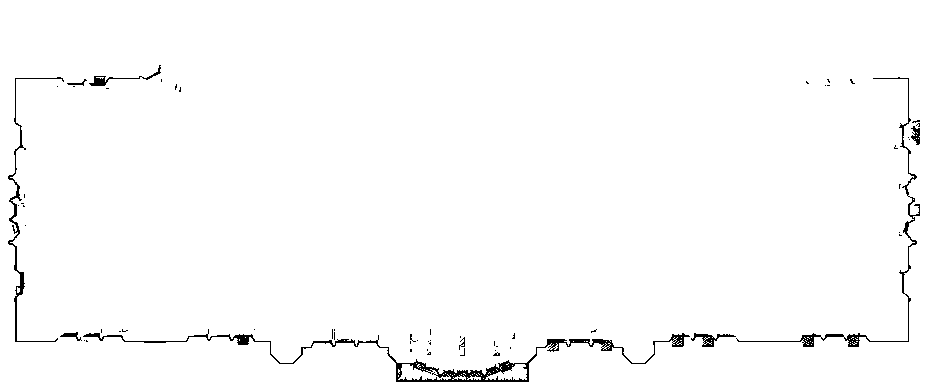
\includegraphics
        [width=2in]
	{figures/image_slice_0190.png}
	}
  }
  \subfloat[]{
    \label{fig_slicing:b} %% label for first subfigure
    \fbox{
    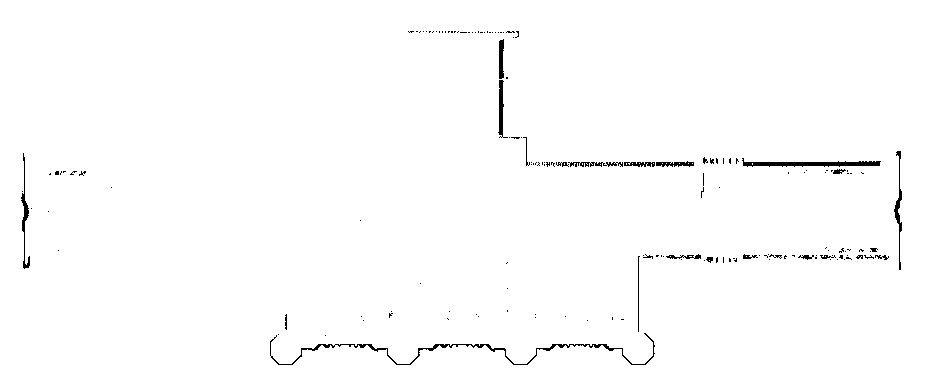
\includegraphics
        [width=2in]
	{figures/image_slice_0714.png}
	}
  }
%  \vspace{.01in}
%  \subfloat[]{
%    \label{fig_slicing:c} %% label for first subfigure
%    \fbox{
%    \includegraphics
%        [width=2in]
%	{figures/image_slice_0886.png}
%	}
%  }
%  \subfloat[]{
%    \label{fig_slicing:d} %% label for first subfigure
%    \fbox{
%    \includegraphics
%        [width=2in]
%	{figures/image_slice_0951.png}
%	}
%  }
  \caption{
The samples of 2D sliced images.
}
  \label{fig_slicing}
\end{figure}

Without loss of generality, the $y-$axis is used to represent the bottom-up
vertical direction.
We project the 3D data
$\boldsymbol{P}(x,y,z), H_{lo} \leq y < H_{hi}$, in the height range
$[H_{lo}, H_{hi})$ onto a 2D image slice.
The projection is normalized in the range $[0,W]$,
where $W$ is the image width:
\begin{equation}\label{eq_image_slicing}
[\,x^{2D},\; y^{2D}\,]^T = \omega\cdot[\,x^{3D}_i - X_{MIN},\; z^{3D}_i - Z_{MIN}\,]^T
\end{equation}
Note that $\omega = W/(X_{MAX} - X_{MIN})$, and that
the [$X_{MIN}$, $X_{MAX}$] and [$Z_{MIN}$, $Z_{MAX}$] pairs define the
3D bounding box, which can be obtained through user input and can be used
to clip away noise data. Fig. \ref{fig_slicing}(a)-(b) show some examples of the
2D slices, where noise and incomplete data are observed.

\subsection{Missing Data Recovery}
\label{sec_mdr}
The slices we extract above are often filled with holes due to occlusion
or other visibility issues.
Fortunately, most urban buildings have symmetry that we can exploit to
fill these holes.
Symmetry computation on 3D data \cite{Sym_PSGRF,Sym_ZPA} is expensive,
so we conduct this computation on the 2D image slices.
Since the 3D data has been already rectified \cite{RDP_LSYGS} and projected onto 2D slices, hence only 2D translation
is needed to be considered for symmetry computation.
Let $P(x,y)$ be a point on the original image $I$ and $P'(x',y')$ be the reflected
point of $P$ with respect to a symmetry line $L$.
The symmetry computation equation for $L$ is as follows:
\begin{equation}
L = \underset{x,y}{\operatorname{arg\,min}}\sum{d_{x,y}(P', I)}
\end{equation}
where the $d_{x,y}(P',I)$ is the distance between the self-reflected point
$P'$ and its nearest data point in image $I$.
The reflected point $P'$ of the original point $P$ is computed with
respect to a line along either the $x-$ or $y-$ axis.
Therefore, the symmetry line $L$ is obtained as the line with minimum
summation error over the reflected data points.

%%%%%%%%%%%%%%%%%%%%%%%%%%%%%%%%
%%%%%%   3D Reconstruction  %%%%
%%%%%%%%%%%%%%%%%%%%%%%%%%%%%%%%
\section{Lightweight 3D Reconstruction}
\label{sec_reconst}
Our 3D reconstruction algorithm is based on \emph{a priori} knowledge that
urban buildings can be created through a series of extrusion and taper
operations on the salient cross-sections contained in the keyslices.
It is therefore critical to identify those salient cross sections upon
which the extrusion and taper operations will apply.
This will be the key step for successful modeling.

\subsection{Extrusion Detection}
\label{sec_ksd}
The 2D image slices of an extruded region are similar to each other.
Thus, to detect an extrusion region one only needs to compute
the similarity between adjacent slices.
The Hausdorff distance is chosen here as the similarity measure.
Let $P_r(x_r, y_r)$ be a data point in a reference image and
let $P_i(x_i, y_i)$ be a data point in a new observed image $I$.
The Hausdorff distance of image $I$ to reference image $I_r$ is defined as:
\begin{equation} \label{eq.hd}
d_H(I, I_r) = \sum_{i=0}^Nd_{min}(P_i, I_r)
\end{equation}
where $d_{min}(P_i, I_r)$ is the minimum distance from data point $P_i$
in image $I$ to the reference image $I_r$.
Alternatively, we can also define the Hausdorff distance, $d_H(I_r, I)$,
from reference image $I_r$ to a new observed image $I$, using the equation \ref{eq.hd}.
These two distances are usually not equal to each other.
As a rule of thumb, one can choose
$d_{HD} = \text{MAX}\{d_H(I, I_r), d_H(I_r, I)\}$ as the Hausdorff distance.
To compute the keyslices, a threshold $\tau_{d}$ is used for the
Hausdorff distance $d_{HD}$.
If $d_{HD} < \tau_{d}$, the two images $I$ and $I_r$ are considered
similar to each other.
Otherwise, a keyslice image is found and $I_r$ is updated with $I$,
the new keyslice image.

\begin{figure}
\centering
%%----start of first figure graphics----
\begin{minipage}[b]{.5\linewidth}
\centering
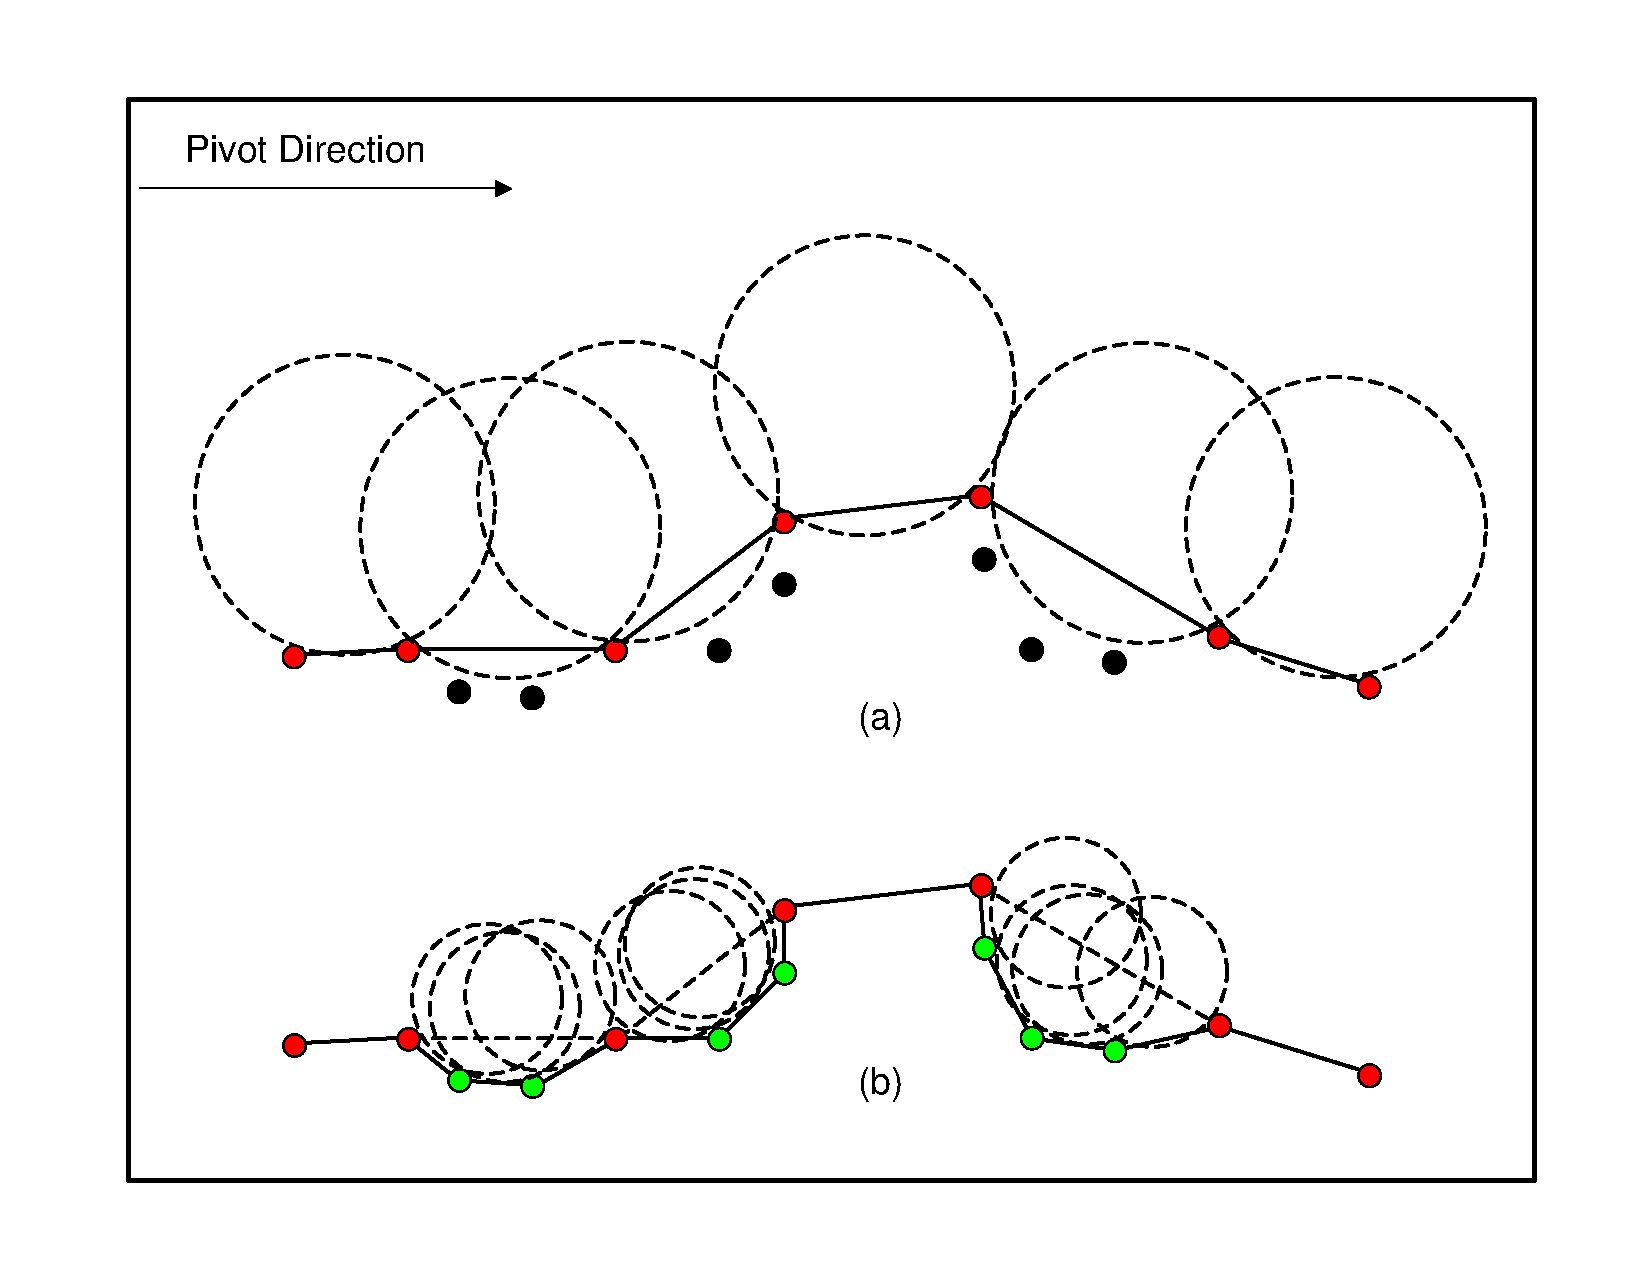
\includegraphics[width=2.7in]{figures/BPA.pdf}
\end{minipage}%
\hspace{1cm}%
%%----start of second figure graphics----
\begin{minipage}[b]{.4\linewidth}
\centering
  \subfloat[]{
    \label{fig_DXF_top:a} %% label for first subfigure
    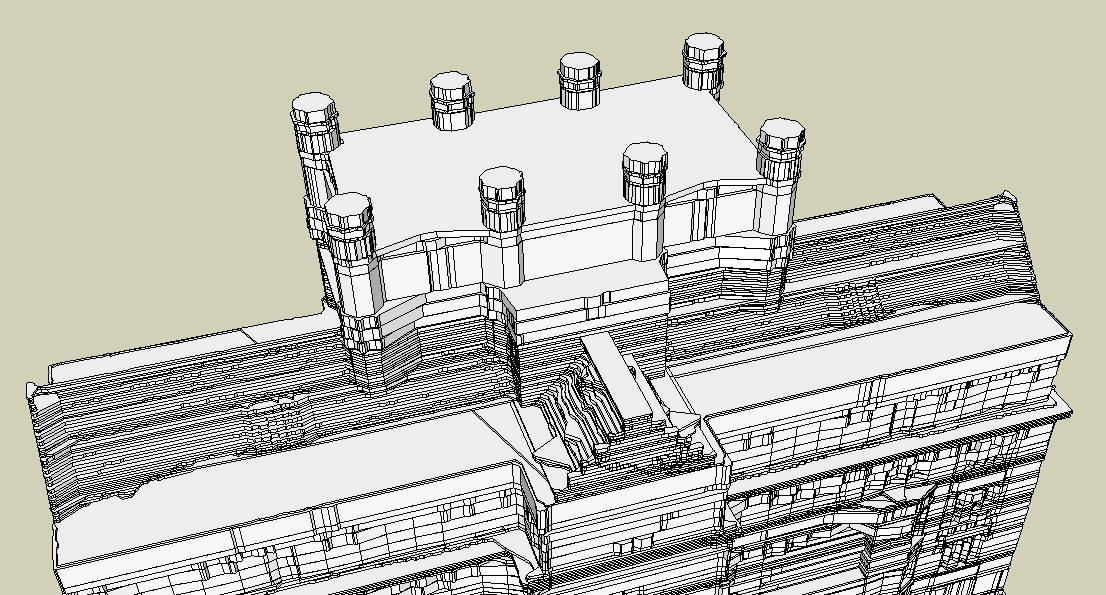
\includegraphics
        [width=1.85in]
	{figures/extrude_1.png}
  }
  \vspace{0.01cm}
  \subfloat[]{
    \label{fig_DXF_top:b} %% label for first subfigure
    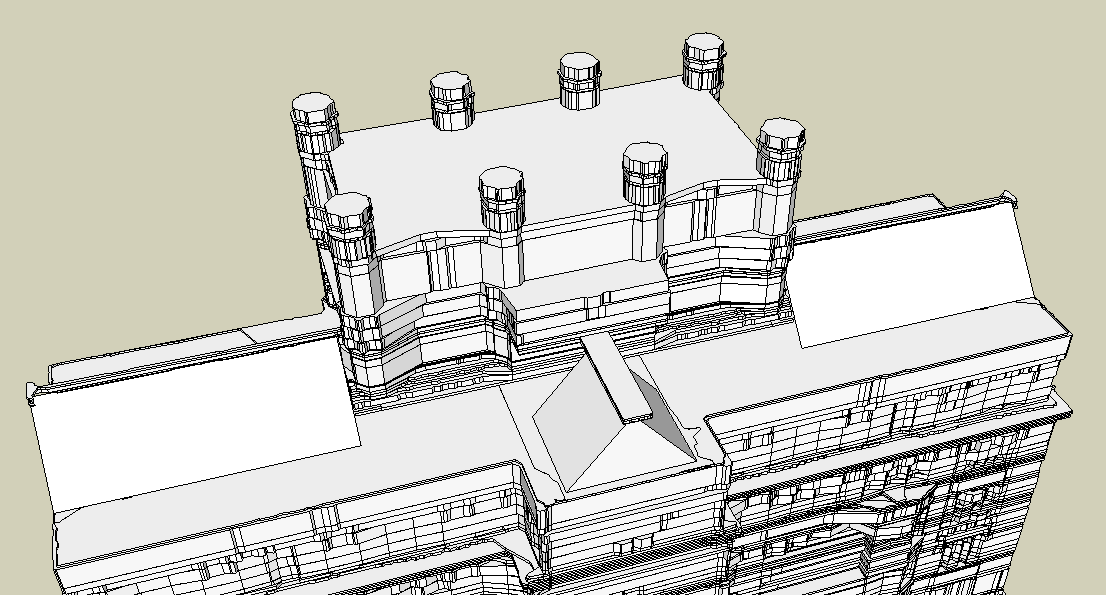
\includegraphics
        [width=1.85in]
	{figures/extrude_2.png}
  }
\end{minipage}
%%----start of first figure caption----
\begin{minipage}[t]{.5\linewidth}
\caption{Ball pivoting: (a) initial pivoting and (b) refinement with smaller radius}
\label{fig_BPA}
\end{minipage}%
\hspace{1cm}%
%%----start of second figure caption----
\begin{minipage}[t]{.4\linewidth}
\caption{Models of (a) no tapered, (b) with tapered structure }
\label{fig_DXF_top}
\end{minipage}%
\end{figure}

The accuracy of the keyslices detected by using the Hausdorff distance
is mainly dependent on the threshold $\tau_d$.
Small $\tau_d$ leads to more accurate models and will require more time and
space to compute and store the result.
Therefore, there is a trade-off between model accuracy and time-space
efficiency.

\subsection{Boundary Vectorization}
After the keyslices are detected, $N_K$ keyslices will be identified
from a total of $N_A$ image slices.
Depending on the threshold $\tau_{d}$, $N_K$ is usually about one to two
orders of magnitude smaller than $N_A$, e.g., $N_K/N_A$ is 0.06 when
$\tau_d$ = 4.0 for the example in
Figure \ref{fig_IR_2_DXF}\subref{fig_IR_2_DXF:a}.
To generate the 3D model, these keyslice images need to be vectorized to
represent the silhouette or boundary of the building.
Several raster image vectorization approaches are proposed in
\cite{DP_AAKMT,DP_DP}.
The Douglas-Peucker algorithm attempts to connect all of the existing points
to form a polygon.
Although the implementation of this approach is very efficient with the
improvement described in \cite{DP_HS}, this method cannot handle the case
where spurious interior points are present, which contributes to outlier data.
To tackle this issue, we adapted the ball-pivoting algorithm (BPA)
\cite{BPA_BMRS} from its original use on 3D point cloud data to use on
2D keyslice images where it produces vectorized boundaries.
The key parameter for the BPA algorithm to work successfully is to
find the right size of the ball for pivoting.
We propose a coarse-to-fine adaptive BPA algorithm, described below,
to solve this problem.

Due to the gap between data points, a relatively large radius $r$ is chosen
as a coarse step to ensure that the ball will travel across all boundary
data before turning back or reaching any existing boundary points.
Figure \ref{fig_BPA}(a) shows an initial ball-pivoting process on 2D
data points.
The output of the initial BPA $\boldsymbol{\Phi}$ contains an ordered list of the boundary data
points $\boldsymbol{P}$ and their corresponding directions $\overrightarrow{\boldsymbol{R}}$ in which
the circle $C$ starts pivoting.
The iterative BPA refinement process is applied on $\boldsymbol{\Phi}$ to get more accurate results with
a smaller radius $r'=r/2$ as shown in Figure \ref{fig_BPA}(b).
The length of each line segment formed by adjacent points
is checked, $\ell = \overline{P_0P_1}$, in $\boldsymbol{\Phi}$.
If this line is long enough, the BPA is applied between the two adjacent points.
When the ball reaches the second point, a new list of ordered boundary points,
$\boldsymbol{\Phi'}$, is inserted into $\boldsymbol{\Phi}$ between $P_0$ and $P_1$.
This process continues until it finishes checking every adjacent point in $\boldsymbol{\Phi}$.
The refinement stops when $r'$ falls below threshold $\tau_r$.

\subsection{Tapered Structure Detection}
\label{sec_tsd}
After the keyslices are detected and vectorized, the silhouettes of
$N_K = \{I_{i}, i = 0, ..., K \}$ keyslices
can be used to represent the whole building based on the extrusion operation.
That is, the space between each pair of keyslices, say $I_{i}$ and $I_{j}$,
can be interpolated by the lower keyslice, e.g., $I_{i}$ in this case.
This is valid due to the similarity between the intermediate images and the
keyslice $I_{i}$.
By modeling a building using this series of keyslices $N_K$, we can largely
reduce the space needed to store urban buildings.
This helps make possible 3D web-based applications such as 3D city navigation.

In addition to the extrusion operation, we can further improve the model
and reduce the model size by observing that part of the keyslice images
belong to the same tapered structure.
This is demonstrated in Figure \ref{fig_DXF_top}.
Figure \ref{fig_DXF_top}\subref{fig_DXF_top:a} shows the roof structure
of the reconstructed model based on a keyslice image extrusion operation with
almost half of the keyslice images dedicated to the roof structure.
After applying the tapered structure inference,
Figure \ref{fig_DXF_top}\subref{fig_DXF_top:b}
shows the improvement of the modeling.
As we can see, the roof in Figure \ref{fig_DXF_top}\subref{fig_DXF_top:b}
is much smoother than that in Figure \ref{fig_DXF_top}\subref{fig_DXF_top:a}.
In addition, the keyslices needed to represent the building, and its
associated storage, are reduced almost in half.

The difficulty of inferring tapered structure lays on the complication of
the building structure itself.
Let's assume that the height range for roof structure is
$H_R = [H_{lo}, H_{hi}]$.
If this is the only existing structure between $H_R$, it is simple and
straight-forward to detect and infer this part.
%Namely, we only need to find the corresponding feature points between the bottom
%the top feature points.
However, for some complicated structures, such as a mixed layout
of tapered and extruded structures, some special treatment is needed to obtain
the desired results.
Our approach is based on the divide and conquer strategy: the whole
structure $\boldsymbol{U}$ is segmented into independent sub-structures,
$U_0, U_1, \ldots, U_N$. For any sub-structure $U_i$,
it contains only a unique structure, either a tapered or an extruded one. Once
each unit $U_i$ is inferred, the whole structure can be modeled by an union operation
of these sub-structures, i.e., $\boldsymbol{U} = \bigcup{U_i\{ i = 1,\ldots,N\}}$.
Before segmentation, the potential height ranges $H_R$ containing the tapered structures should be computed.
This can be done by checking the frequency of the keyslice images.
The structure containing tapered sub-structures will show a high and even
distributed keyslice images. This is a very useful clue for $H_R$ detection.

%%% Figure of the tapered template.
\begin{figure} [!btp]
  \subfloat[]{
    \label{fig_IN:a} %% label for first subfigure
    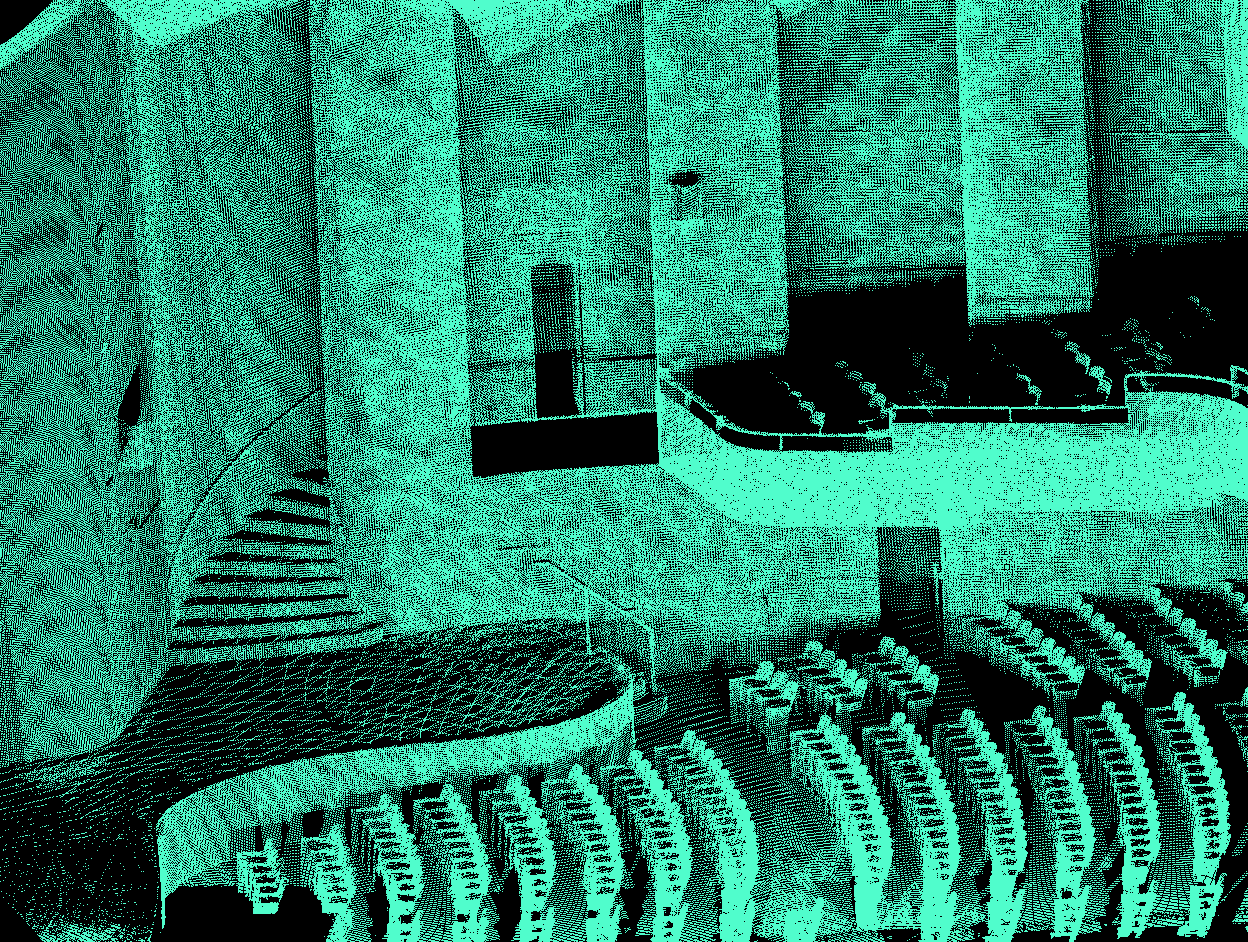
\includegraphics
        [width=2in]
	{figures/range_crop.png}
  }
  \centering
  \subfloat[]{
    \label{fig_IN:b} %% label for first subfigure
    \includegraphics
        [width=2in]
	%{figures/model_crop.png}
	{figures/HunterTheatreShaded.jpg}
  }
  \caption{The model of an interior scanning. (a) The snapshot of the interior scanning point cloud data.
(b) the model reconstructed from the interior scanning.}
  \label{fig_IN}
\end{figure}
%%% End of Figure

Once the potential height ranges $H_R$ is obtained,
the next step is to segment the whole structure $\boldsymbol{U}$ between $H_R$ into
sub-structures, $U_i, \; i = 0,\ldots,N$. This is again done by similarity measurement of sliced images
from orthogonal directions. As before, the 3D data points following inside the range of $H_R$
are projected along both left-right ($X$ axis) and face-inside ($Z$ axis) directions.
Then the keyslice detection is carried out based on Hausdorff distance similarity measurement for
both directions. These keyslices will segment the structure in $H_R$ into sub units of $U_0, U_1, \ldots, U_N$.

For each sub unit $U_i$, we have to know whether it represents an extruded or a tapered
structure. The method is to check in the keyslice image $I_k$ of $U_i$ whether there exists
a pattern where two lines intersect with some appropriate angle.
% as shown in Figure \ref{TSD_fig_tapered_template}.
If such a pattern exists in $I_k$, the
unit $U_i$ is marked as a tapered sub-structure. Otherwise, $U_i$ is marked as
an extruded sub-structure. If $U_i$ is an extruded unit, its silhouette from the
$y-$ axis is vectorized and is ready for the union operation to obtain $\boldsymbol{U}$.
On the other hand, if $U_i$ is a tapered unit, the bottom and top position have to be computed
so that it can be reconstructed. To do this, all line segments $\boldsymbol{L}$ in $U_i$
are computed using the Hough Transform and the
%described in Algorithm \ref{alg.AHT}.
intersection point $P_0$ of $\boldsymbol{L}$ indicates
the top position of the tapered unit. The other end points $P_i$ of $\boldsymbol{L}$ are also computed
to infer the bottom shape and position.

%%%%%%%%%%%%%%%%%%%%%%%%%%%%%%%%
%%%%%%   Experimental Results%%%
%%%%%%%%%%%%%%%%%%%%%%%%%%%%%%%%
\section{Experimental Results and Conclusion}
\label{sec_IR_OUT}
The results of the extrusion and tapered structures computation,
together with raster image vectorization, are stored in the 2D
image coordinate system. To generate the final 3D model, these
data need to be transformed
back into the 3D world coordinate system.
Let $P(x,y)$ be a point in the 2D image coordinate system, and let
$P'(x,y,z)$ be the 3D world coordinate of $P$, where $y$ is the depth coordinate.
For all points in the same boundary layer or silhouette,
the points lay in the same plane and hence have the same value of $y$.
The equation for transforming $P$ back to $P'$ is a reverse transformation of $\boldsymbol{T_0}$
in the equation \ref{eq_image_slicing}:
\begin{equation}\label{eq_ir2dxf}
[\,x^{3D},\; y^{3D},\; z^{3D}\,]^T = [\,\eta\cdot x^{2D} + X_{MIN},\; \zeta + Y_{MIN},\; \eta\cdot z^{2D} + Z_{MIN}\,]^T
\end{equation}
where $\eta=1/\omega$ and $\zeta=\kappa\cdot\delta$. Here, $\kappa$ is the index of the 2D slice and $\delta$
is the height of a slab described in the Section \ref{sec_image_slicing}.
Figure \ref{fig_IR_2_DXF}\subref{fig_IR_2_DXF:d} shows an exterior 3D model
generated by the above transformation.
In addition to the exterior model, we have also applied the approach on
the range data of an interior scanning.
The snapshot of this interior scan is shown in Figure \ref{fig_IN}\subref{fig_IN:a}
and its reconstructed 3D model is shown in Figure \ref{fig_IN}\subref{fig_IN:b}.
This model is primarily reconstructed using the extrusion unit, and the
chairs and some fine details are ignored. However, the
main structures of the interior are captured and the chairs can be added to
the model through texture mapping.
Please note that the model generated in  Figure \ref{fig_IN}\subref{fig_IN:b}
is of low resolution and some details may lost, which can be captured by using
a smaller threshold $\tau_d$ to obtain higher resolution models.

\setlength{\tabcolsep}{4pt}
\begin{table}[btp]
\begin{center}
\caption{The error measurement with respected to Hausdorff distance threshold $\tau_d$.
The BPA radius threshold $\tau_r = 4$}
\label{tbl_em}
  \begin{tabular}[t]{||c||c|c|c||}
    \hline
    $\tau_{d} $(pixel) & Error (mm)& \# of faces & Size (KB) \\
    \hline \hline
    64 & 0.658 & 1471 & 15\\   %   64 & 9.63 & 1471 & 15\\
    \hline		      %   \hline		
    32 & 0.294 & 3284 & 32\\   %   32 & 4.30 & 3284 & 32\\
    \hline		      %   \hline		
    16 & 0.141 & 8574 & 86\\   %   16 & 2.06 & 8574 & 86\\
    \hline		      %   \hline		
    8 & 0.131 & 13955 & 137\\  %   8 & 1.91 & 13955 & 137\\
    \hline		      %   \hline		
    4 & 0.094 & 27214 & 261\\  %   4 & 1.38 & 27214 & 261\\
    \hline		      %   \hline		
    2 & 0.088 & 31331 & 335\\  %   2 & 1.28 & 31331 & 335\\
    \hline
  \end{tabular}
\end{center}
\end{table}
\setlength{\tabcolsep}{1.4pt}
To measure the error of a reconstructed 3D model,
we first transform it to the 3D point cloud coordinate system.
The error is measured as the distance from the sampled 3D points to their closest model planes, which
is computed using the following formula:
\begin{equation}\label{eq_em}
E = \frac{1}{|X|}\sum_{x\in{X}}{d^2(x, M)}
\end{equation}
where $X$ is the set of 3D point cloud data. The distance
$d(x, M) = \text{min}_{p \in M}\lVert x - p \lVert$ is the minimum Euclidean distance from
a 3D point $x$ to its closest face $p$ of $M$.
%%% Figure of the tapered template.
\begin{figure} [!btp]
  \subfloat[]{
    \label{fig_EM:a} %% label for first subfigure
    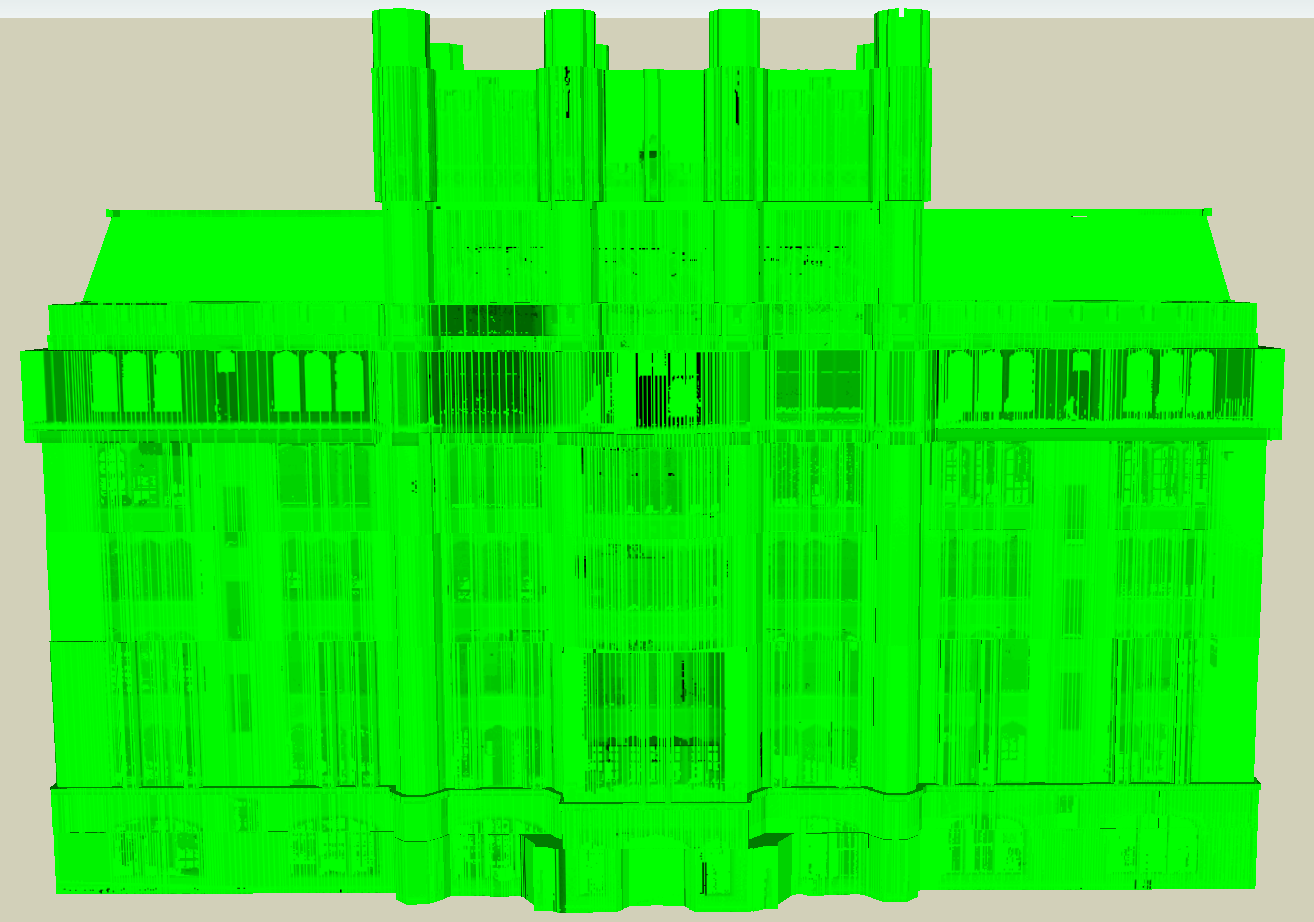
\includegraphics
        [width=2in]
	{figures/IR_skp_error_face_1000_32_4_paper.png}
  }
  \centering
  \subfloat[]{
    \label{fig_EM:b} %% label for first subfigure
    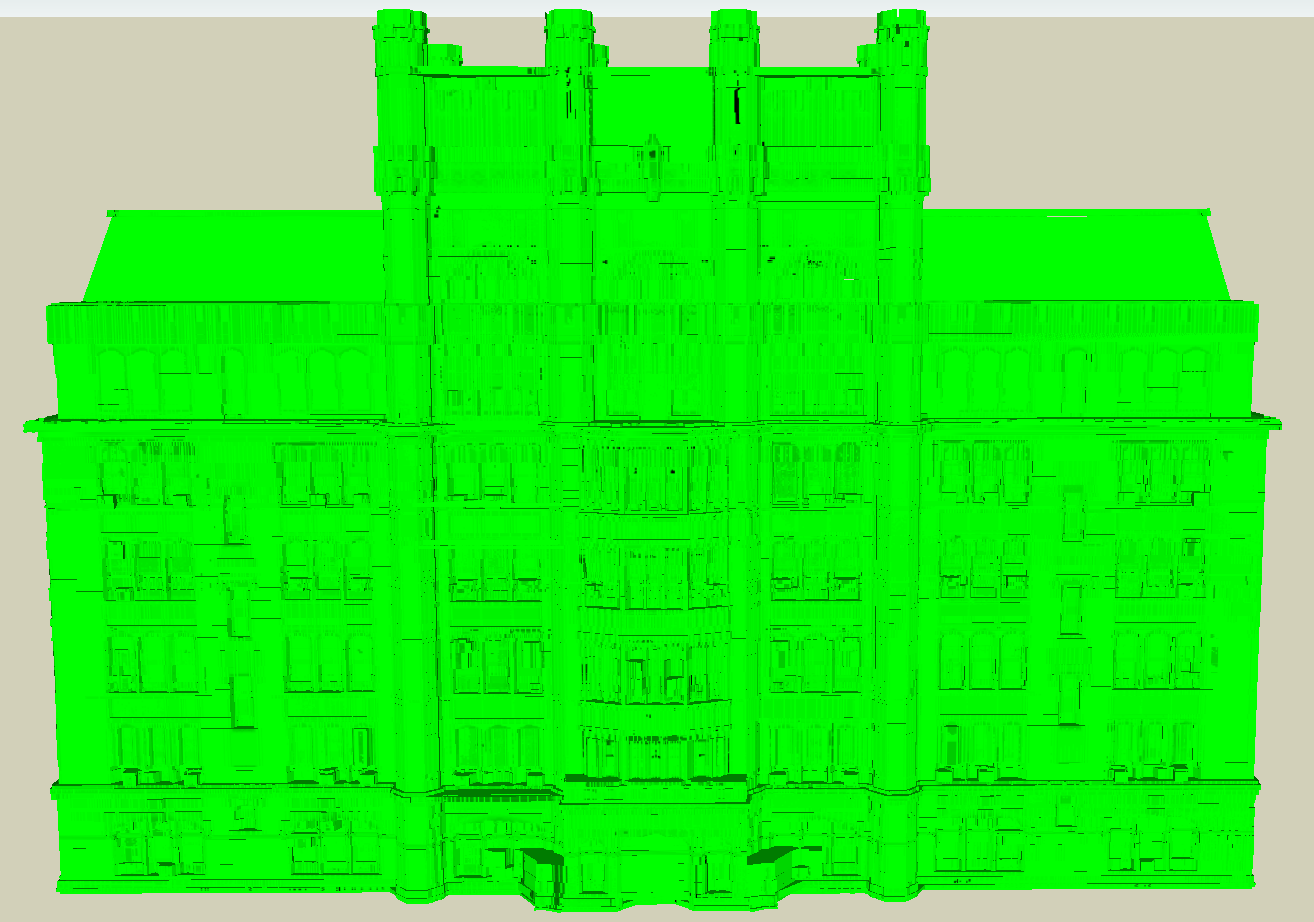
\includegraphics
        [width=2in]
	{figures/IR_skp_error_face_1000_4_1_paper.png}
  }
  \caption{  The deviation mapping of the 3D point cloud. (a) the result with $\tau_r$ = 4 and $\tau_d$ = 32.
(b) the result with $\tau_r$ = 1 and $\tau_d$ = 4. }
  \label{fig_EM}
\end{figure}
%%% End of Figure
To visualize the error between real 3D data and the inferred model,
we generated the deviation mapping images which are depicted in Figure \ref{fig_EM}.
Basically, for each face $p$ of $M$, a corresponding texture image is computed. 
The intensity of each pixel in the texture image
is determined by the error of the corresponding 3D points computed by Equation \ref{eq_em}.
The accuracy of the reconstructed model is mainly controlled by the threshold of Hausdorff distance $\tau_d$
and BPA refinement radius $\tau_r$. $\tau_d$ determines the accuracy of the keyslice detection
and $\tau_r$ determines the accuracy of the boundary vectorization.
Table \ref{tbl_em} lists the relationship among the $\tau_d$, errors, number of faces and model size.
The unit for $\tau_d$ is in pixels and for errors is in millimeters.
The size for original 3D building point cloud is more than 700 MB. From the table, one can see that even
for the most accurate model, the size is dramatically reduced compared with the original 3D point cloud data,
which is desired for web-based applications (Fig. \ref{fig_GE}).

In conclusion, we presented a lightweight 3D modeling of urban buildings from range data.
Our work is based on the observation that buildings can be
viewed as the combination of two basic components, the extrusion and
the tapering components.
The efficient and economical techniques proposed here are used to infer
the extruded and tapered unit, and then reconstruct the 3D model
via vectorization.
The experimental results on both exterior and interior urban building datasets
are presented to validate the proposed approach.

\bibliographystyle{splncs}
\bibliography{accv}

\end{document}
